%
% section 3.1.2
%
\subsection{Κλάσεις (Τάξεις) Δικτύων -- Διευθύνσεων}

Μια διεύθυνση δικτύου αποτελείται πάντα από δύο τμήματα: το πρώτο τμήμα \emph{αναγνωρίζει το δίκτυο} στο οποίο ανήκει ο υπολογιστής (Network ΙD ή πρόθεμα - prefix) και το δεύτερο μέρος αναγνωρίζει τον υπολογιστή (Host ID ή επίθεμα - suffix) μέσα στο συγκεκριμένο δίκτυο. Αν θέλουμε να κάνουμε μια αντιστοίχιση με την καθημερινότητα, το τμήμα δικτύου δείχνει την οδό στην οποία βρίσκεται μια κατοικία ενώ το τμήμα υπολογιστή είναι ο αριθμός της πάνω στην οδό.

Για παράδειγμα, στην διεύθυνση 192.168.1.12, το τμήμα δικτύου είναι το 192.168.1 και δείχνει στο δίκτυο 192.168.1.0 ενώ το τμήμα υπολογιστή είναι το 12, που προσδιορίζει ένα συγκεκριμένο υπολογιστή πάνω σε αυτό το δίκτυο.

\begin{center}
  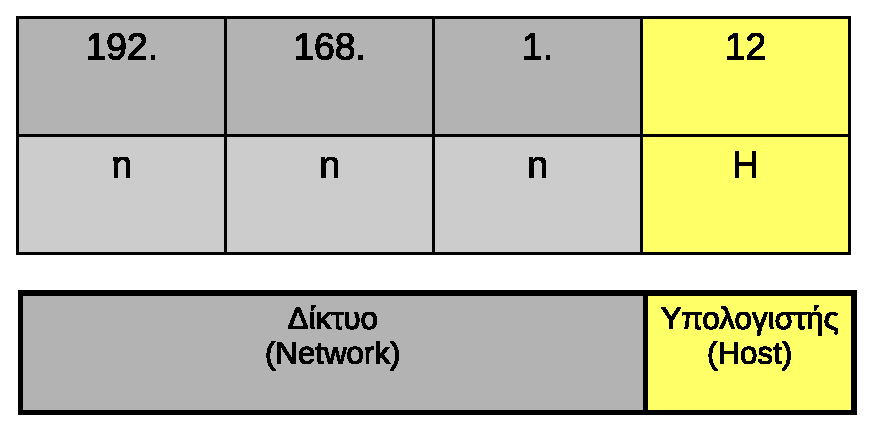
\includegraphics[width=0.55\textwidth]{images/chapter3/3-2}
\end{center}

Τα δύο αυτά τμήματα δεν καταλαμβάνουν το ίδιο μήκος: διαφοροποιούνται ανάλογα με το μέγεθος του δικτύου και το πλήθος των υπολογιστών που θέλουμε να συνδέσουμε σε αυτό. Στο παράδειγμα μας, το τμήμα υπολογιστή χρησιμοποιεί μόνο την τελευταία οκτάδα (το τελευταίο byte) της διεύθυνσης. Με 8 bit μπορούμε να γράψουμε μέχρι 2\textsuperscript{8}=256 διαφορετικές διευθύνσεις, άρα στο δίκτυο 192.168.1.0 μπορούμε να συνδέσουμε μέχρι 256 διαφορετικούς υπολογιστές (στην πραγματικότητα 254, καθώς η τιμή 0 προσδιορίζει τη \emph{διεύθυνση δικτύου} και το 255 την \emph{διεύθυνση εκπομπής} του δικτύου και δεν μπορούν να χρησιμοποιηθούν για κανονικές διευθύνσεις μηχανημάτων).

Αν θέλουμε το δίκτυο να έχει περισσότερους από 254 υπολογιστές, θα πρέπει να δώσουμε στο τμήμα υπολογιστή ακόμα μια οκτάδα. Τότε το δίκτυο θα μπορεί να έχει μέχρι 2\textsuperscript{16}=65536 υπολογιστές (στην πραγματικότητα, 65535 - 2 = 65534 όπως και πριν). Για ακόμα μεγαλύτερα δίκτυα μπορούμε να δώσουμε ακόμα μια οκτάδα στο τμήμα υπολογιστή, φτάνοντας έτσι τα 24 bit για το τμήμα υπολογιστή.  Όσο αυξάνουμε το ένα τμήμα της διεύθυνσης IP, ανάλογα μειώνεται το άλλο και συνολικά η διεύθυνση παραμένει πάντα 32 bit. 

Με τον παραπάνω τρόπο ορίζουμε \emph{τάξεις ή κλάσεις} δικτύων ανάλογα με το μέγεθος που μας εξυπηρετεί: ουσιαστικά μπορούμε να φτιάξουμε λίγα δίκτυα με μεγάλο αριθμό υπολογιστών (όταν δώσουμε τρεις οκτάδες στο τμήμα υπολογιστή), περισσότερα δίκτυα με ενδιάμεσο αριθμό υπολογιστών (όταν δώσουμε δύο οκτάδες στο τμήμα υπολογιστή) ή πολλά δίκτυα με λίγους υπολογιστές (όταν δώσουμε μια οκτάδα στο τμήμα υπολογιστή). Ο πίνακας στο σχήμα \ref{3-2} δείχνει αυτούς τους συνδυασμούς.

\begin{figure}[!ht]
  \centering
  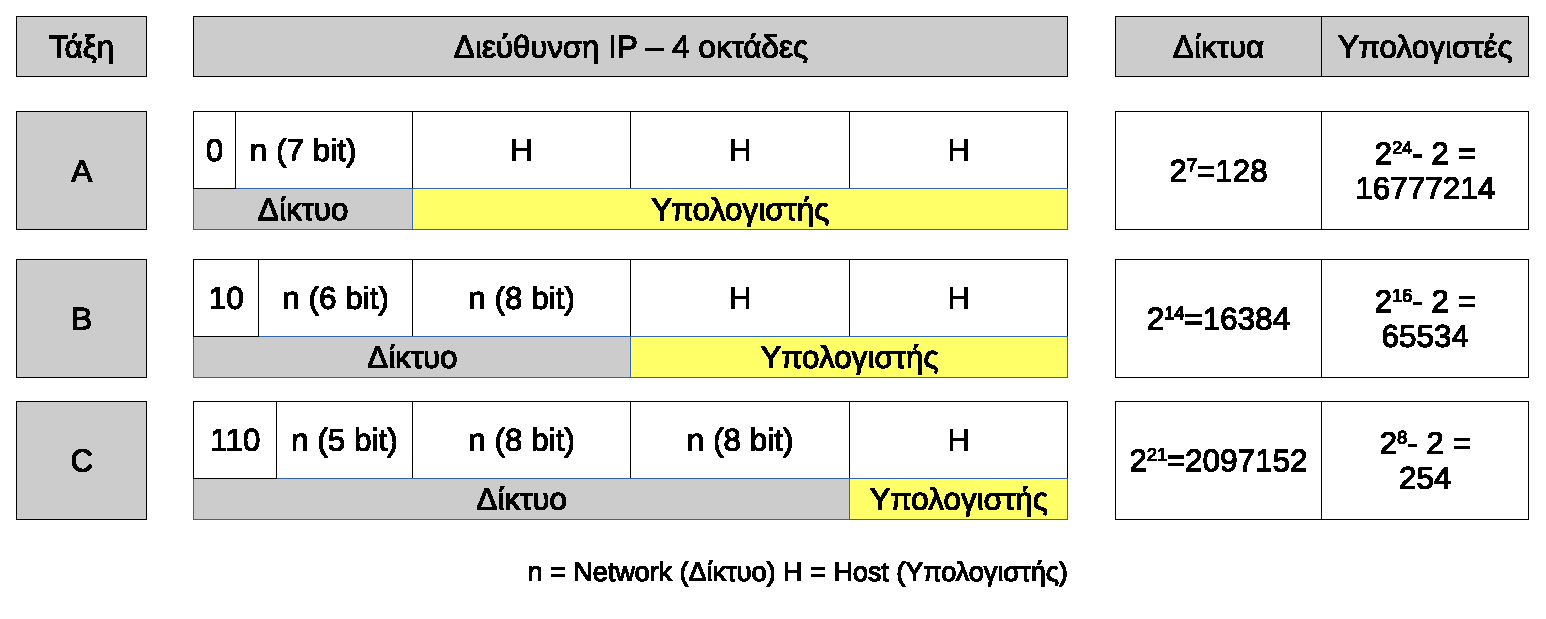
\includegraphics[width=0.95\textwidth]{images/chapter3/3-3}
  \caption {\textsl{Κλάσεις/Τάξεις Διευθύνσεων IPv4}}
  \label{3-2}
\end{figure}

Συνολικά οι τάξεις δικτύων που μας ενδιαφέρουν είναι τρεις και χαρακτηρίζονται με τα γράμματα A,B,C. Προσέξτε ότι ανάλογα με την κλάση ορίζεται κάποιο ή κάποια ψηφία στην πρώτη οκτάδα που έχουν συγκεκριμένη τιμή. Έτσι:

\begin{itemize}
\item \textbf{Για Δίκτυα Τάξης Α:} Το πρώτο ψηφίο της πρώτης οκτάδας \textbf{έχει την τιμή 0}. Έτσι η πρώτη οκτάδα παίρνει τιμές από 00000000 μέχρι 01111111 δηλ. από 0 ως 127.
\item \textbf{Για Δίκτυα Τάξης Β:} Τα δύο πρώτα ψηφία της πρώτης οκτάδας \textbf{έχουν την τιμή 10}. Έτσι η πρώτη οκτάδα παίρνει τιμές από 10000000 μέχρι 10111111 δηλ. από 128 ως 191.
\item \textbf{Για Δίκτυα Τάξης C:} Τα τρία πρώτα ψηφία της πρώτης οκτάδας \textbf{έχουν την τιμή 110}. Έτσι η πρώτη οκτάδα παίρνει τιμές από 11000000 μέχρι 11011111 δήλ. από 192 ως 223.
\end{itemize}

Εκτός από τις A,B,C που χρησιμοποιούνται για κανονική διευθυνσιοδότηση σε δίκτυα υπάρχουν και οι τάξεις D (διευθύνσεις που χρησιμοποιούνται για πολυδιανομή - multicasting) και Ε (δεσμευμένες) οι οποίες όμως είναι ειδικού σκοπού και δεν χρησιμοποιούνται ως διευθύνσεις σε υπολογιστές δικτύων.  Ο πίνακας \ref{t3-1-2} συνοψίζει τις τάξεις διευθύνσεων και τα χαρακτηριστικά τους.

\begin{table}
\centering
  \begin{tabular}{|c|c|c|c|c|c|c|c|}
    \rowcolor[gray]{0.95}
    \hline
    \multirow{2}{*}{} Τάξη & 1η Οκτάδα & \multicolumn{2}{|c|}{Δυαδικό} & \multicolumn{2}{|c|}{Δεκαδικό} & Παρατηρήσεις \\ 
    \cline{3-6}
     \rowcolor[gray]{0.95}
    & & Από & Έως & Από & Έως & \\
    \hline
    A & 0xxx xxxx & 0000 0000 & 0111 1111 & 0 & 127 & x: 0 ή 1\\
    \hline
    Β & 10xx xxxx & 1000 0000 & 1011 1111 & 128 & 191 & \\
    \hline
    C & 110x xxxx & 1100 0000 & 1101 1111 & 192 & 223 & \\
    \hline
    \multirow{2}{*}{}D & 1110 xxxx & 1100 0000 & 1110 1111 & 224 & 239 & Multicast  \\
    & & & & & & (Πολυδιανομή) \\
    \hline
    E & 1111 0xxx & 1111 0000 & 1111 1111 & 240 & 255 & Δεσμευμένες\\
    \hline 
  \end{tabular}
  
\caption{Προσδιορισμός Κλάσης/Τάξης Διευθύνσεων}
\label{t3-1-2}
\end{table}

Κοιτάζοντας μόνο τη τιμή της πρώτης οκτάδας, μπορούμε άμεσα να προσδιορίσουμε σε ποια κλάση ανήκει το δίκτυο:

\begin{itemize}
\item Από 1 - 127: Δίκτυο τάξης Α
\item Από 128 - 191: Δίκτυο τάξης B
\item Από 192 - 223: Δίκτυο τάξης C
\item Τιμές από 224 και άνω είναι ειδικού σκοπού (όχι για απόδοση διεύθυνσης δικτύου σε υπολογιστή)
\end{itemize}

Εννοείται ότι αν μας δίνουν τη διεύθυνση στο δυαδικό, κοιτάζουμε την τιμή των πρώτων ψηφίων της πρώτης οκτάδας!
Ο παρακάτω πίνακας δίνει παραδείγματα διευθύνσεων και τάξεων που ανήκουν:

\begin{center}
\begin{tabular}{|c|c|c|}
\hline
\rowcolor[gray]{0.95}
Διεύθυνση IP & Τάξη & Αιτιολογία \\
\hline
192.168.1.12 & C & Το 192 ανήκει στο διάστημα 192\ldots223\\
\hline
10.146.0.1 & A & Το 10 ανήκει στο διάστημα 0\ldots127\\
\hline
172.16.32.253 & B & Το 172 ανήκει στο διάστημα 128\ldots191\\
\hline
127.0.0.1 & A & Το 127 ανήκει στο διάστημα 1\ldots127\\
\hline
194.219.227.1 & C & Το 194 ανήκει στο διάστημα 192\ldots223\\
\hline
\end{tabular}
\end{center}

\subsubsection*{Διαχείριση και Απόδοση Διευθύνσεων IP}

Οι διευθύνσεις IP είναι μοναδικές στον κόσμο: Ανά πάσα στιγμή δεν είναι δυνατόν δύο υπολογιστές με άμεση σύνδεση στο Internet να έχουν την ίδια διεύθυνση IP. Η διαχείριση των διευθύνσεων γίνεται από ένα κεντρικό φορέα, τον \emph{IANA/ICANN} (\href{http://www.iana.org}{Internet Assigned Numbers Authority} και \href{https://www.icann.org}{Internet Corporation for Assigned Names and Numbers}). Ο φορέας αυτός μεταβιβάζει αρμοδιότητες διαχείρισης σε περιφερειακούς καταχωρητές (RIR -- Regional Internet Registry) και μέσω αυτών σε τοπικούς ή εθνικούς καταχωρητές (LIR -- Local Internet Registry ή NIR -- National Internet Registry). Για την Ευρώπη, Μέση Ανατολή και Κεντρική Ασία περιφερειακός καταχωρητής Internet είναι το \href{https://www.ripe.net/}{RIPE NCC}.

Οι τελικοί απλοί (οικιακοί) χρήστες καθώς και εταιρικοί χρήστες απευθύνονται στον πάροχο υπηρεσιών Διαδικτύου (ISP, Internet Service Provider) ο οποίος παρέχει υπηρεσίες πρόσβασης στο Διαδίκτυο και αποδίδει κάθε φορά σε αυτούς τις απαιτούμενες διευθύνσεις IP. Η απόδοση μπορεί να γίνεται δυναμικά (π.χ. αν κλείσουμε τον οικιακό μας δρομολογητή ADSL και τον ξανανοίξουμε, θα πάρουμε μια διαφορετική IP διεύθυνση) ή στατικά (να παίρνουμε κάθε φορά την ίδια σταθερή IP). Οι IPSs συνήθως είναι και τοπικοί καταχωρητές.

\subsubsection*{Ιδιωτικές Διευθύνσεις IP}

Σύμφωνα με όσα γράψαμε παραπάνω, φαίνεται ότι είναι απαραίτητο πριν φτιάξουμε ένα δίκτυο (ακόμα και για δική μας χρήση) να έχουμε ζητήσει να μας διατεθούν διευθύνσεις IP από κάποιο πάροχο. Ωστόσο αυτό δεν είναι αλήθεια: τα περισσότερα τοπικά δίκτυα υπολογιστών μπορούν να χρησιμοποιούν την τεχνολογία IP αλλά δεν είναι άμεσα συνδεδεμένα στο Internet.

\begin{inthebox}
\textbf{Για παράδειγμα:}

Στο σπίτι σας πιθανότητα διαθέτετε μια σύνδεση ADSL και συνδέεστε με ένα ή περισσότερους υπολογιστές μέσω Ethernet ή WiFi σε ένα δρομολογητή που σας έχει προμηθεύσει ο παροχέας σας. Ο δρομολογητής αυτός αποστέλλει και όλες τις απαραίτητες ρυθμίσεις δικτύου στο μηχάνημα σας (μέσω του πρωτοκόλλου DHCP που θα δούμε σε επόμενη ενότητα) και έτσι δεν χρειάζεται να τις κάνετε εσείς. Αν δείτε τη διεύθυνση IP του μηχανήματος σας, θα διαπιστώσετε ότι είναι της μορφής 192.168.0.X ή 192.168.1.X όπου το Χ αναφέρεται στο τμήμα υπολογιστή.

Οι διευθύνσεις αυτές δεν είναι μοναδικές: όλοι οι οικιακοί δρομολογητές χρησιμοποιούν τις ίδιες ρυθμίσεις. Πως όμως συνδέεστε στο Internet χωρίς μοναδική IP; Στην πραγματικότητα αυτή η διεύθυνση είναι γνωστή μόνο στο δικό σας τοπικό δίκτυο. Ο δρομολογητής διαθέτει δική του διαφορετική (και μοναδική) διεύθυνση με την οποία είναι συνδεδεμένος στο Internet. Η διεύθυνση αυτή αποδίδεται δυναμικά (συνήθως) από τον παροχέα και μπορεί να αλλάζει ανά τακτά διαστήματα (αλλάζει επίσης αν κλείσετε το router και το ξανανοίξετε). Όταν επικοινωνείτε με το Internet, o δρομολογητής αλλάζει τη δική σας εσωτερική διεύθυνση με τη δική του πριν στείλει τα πακέτα σας. Εσωτερικά κρατάει ένα πίνακα αντιστοιχιών ώστε όταν λάβει απάντηση να αλλάξει την διεύθυνση προορισμού ξανά με τη δική σας εσωτερική IP. Η τεχνική αυτή ονομάζεται \emph{NAT (Network Address Translation)} και μας επιτρέπει να συνδέσουμε ένα πλήθος υπολογιστών στο διαδίκτυο ενώ χρησιμοποιούμε μόνο μια δεσμευμένη διεύθυνση IP. Η σύνδεση εδώ δεν είναι άμεση: κανένα από αυτά τα μηχανήματα δεν φαίνεται απευθείας μέσω Internet. Μόνο ο δρομολογητής είναι άμεσα ορατός.\\
\end{inthebox}

Για το σκοπό αυτό έχουν προβλεφθεί περιοχές διευθύνσεων και των τριών τάξεων που μπορούν να χρησιμοποιηθούν αυθαίρετα και χωρίς κανένα συντονισμό με κάποια από τις αρχές διαχείρισης διευθύνσεων. Να σημειωθεί εδώ ότι όλοι οι δρομολογητές της αγοράς είναι από πριν ρυθμισμένοι να αναγνωρίζουν τις περιοχές αυτές και ποτέ δεν δρομολογούν αυτές τις διευθύνσεις στο Internet. Οι περιοχές αυτές περιγράφονται στο έγγραφο \href{https://www.ietf.org/rfc/rfc1918.txt}{RFC1918} - Address Allocation for Private Internets και φαίνονται στον παρακάτω πίνακα:

\begin{center}
\begin{tabular}{|c|c|c|c|}
\hline
\textbf{Τάξη} & \textbf{Από} & \textbf{Εώς} & \textbf{Μορφή CIDR} \\
\hline
A & 10.0.0.0 & 10.255.255.255 & 10.0.0.0/8\\
\hline
B & 172.16.0.0 & 172.31.255.255 & 172.16.0.0/12\\
\hline
C & 192.168.0.0 & 192.168.255.255 & 192.168.0.0/16\\
\hline
\end{tabular}
\end{center}

\textbf{Σημείωση:} Για τη μορφή CIDR θα μιλήσουμε σε επόμενη ενότητα.

Για την υλοποίηση ενός ιδιωτικού δικτύου επιλέγονται διευθύνσεις μόνο από τον παραπάνω πίνακα, ανάλογα με το μέγεθος του δικτύου που θα υλοποιηθεί. Για το τοπικό οικιακό ή μικρό δίκτυο επιλέγονται συνήθως διευθύνσεις από την τάξη C, έτσι συχνά βλέπουμε IP όπως 192.168.0.1 κλπ.
